% REMEMBER: You must not plagiarise anything in your report. Be extremely careful.

\documentclass{l4proj}

    
%
% put any additional packages here
%

\begin{document}

%==============================================================================
%% METADATA
\title{Adaptive Comparative Judgement in JavaScript}
\author{Aisling Chan}
\date{April 17, 2023}

\maketitle

%==============================================================================
%% ABSTRACT
\begin{abstract}

    The traditional method of marking coursework involves assigning points to a piece of work according to a rubric. An alternative method of assessment as emerged in recent years called Adaptive Comparative Judgement (ACJ). Studies have found ACJ to be a very reliable way of evaluating students' work. The assessing coursework using ACJ can be quite time-consuming but software can be used to streamline the process. This project aims to create a web application that facilitates the marking of student work using ACJ. An open source ACJ project written in PHP already exists. This project aims to implement ACJ in JavaScript as it is more widely used.
    
\end{abstract}

%==============================================================================

% EDUCATION REUSE CONSENT FORM
% If you consent to your project being shown to future students for educational purposes
% then insert your name and the date below to  sign the education use form that appears in the front of the document. 
% You must explicitly give consent if you wish to do so.
% If you sign, your project may be included in the Hall of Fame if it scores particularly highly.
%
% Please note that you are under no obligation to sign 
% this declaration, but doing so would help future students.
%
%\def\consentname {My Name} % your full name
%\def\consentdate {20 March 2018} % the date you agree
%
\educationalconsent


%==============================================================================
\tableofcontents

%==============================================================================
%% Notes on formatting
%==============================================================================
% The first page, abstract and table of contents are numbered using Roman numerals and are not
% included in the page count. 
%
% From now on pages are numbered
% using Arabic numerals. Therefore, immediately after the first call to \chapter we need the call
% \pagenumbering{arabic} and this should be called once only in the document. 
%
% Do not alter the bibliography style.
%
% The first Chapter should then be on page 1. You are allowed 40 pages for a 40 credit project and 30 pages for a 
% 20 credit report. This includes everything numbered in Arabic numerals (excluding front matter) up
% to but excluding the appendices and bibliography.
%
% You must not alter text size (it is currently 10pt) or alter margins or spacing.
%
%
%==================================================================================================================================
%
% IMPORTANT
% The chapter headings here are **suggestions**. You don't have to follow this model if
% it doesn't fit your project. Every project should have an introduction and conclusion,
% however. 
%
%==================================================================================================================================
\chapter{Introduction}

% reset page numbering. Don't remove this!
\pagenumbering{arabic} 

\section{Motivation}
Typically markers assess the quality of coursework by allotting a certain number of points based on whether the coursework has met a predetermined set of criteria. This style of marking aims to determine the objective quality of a piece of academic work. The objective nature of this style aims to give an unbiased assessment of the work. This type of marking works well for objective subjects like mathematics or physics. However, this manner of marking is less reliable for work that is more subjective. For work like a musical composition, a piece of creative writing, or a video presentation, it is much harder to reliably judge its quality. This has prompted research into other methods of marking.

In recent years, Adaptive Comparative Judgement (ACJ) has emerged as an alternative method of evaluating students’ coursework. It involves an evaluator being asked to compare two pieces of work and selecting which one is “better”. An ordered ranking of the pieces of coursework can then be created from these comparisons. This ranking can be used to generate coursework grades. Studies have found that ACJ can be used to achieve high levels of reliability and could be used as an alternative to traditional marking strategies \citep{inproceedings, doi:10.1080/0969594X.2013.868341} . It also has the potential to be an effective learning tool for students when used to conduct peer marking \citep{bartholomew2019using}. ACJ has already been used by the University of Glasgow for a variety of assessed exercises within courses on computing science and psychology.

The process of retrieving pairs of coursework, recording which ones are “better”, and ranking all of the work based on the comparisons can be extremely time-consuming if done manually. Therefore, developing software to streamline the process of ACJ marking is crucial to promoting its use within a wider, practical setting.

An open source implementation of ACJ has already been written by \citet{nbarr:code} in PHP. Developing implementations in more popular and more widely deployed languages, such as JavaScript, can further promote the use and development of ACJ.


\begin{figure}
    \centering
    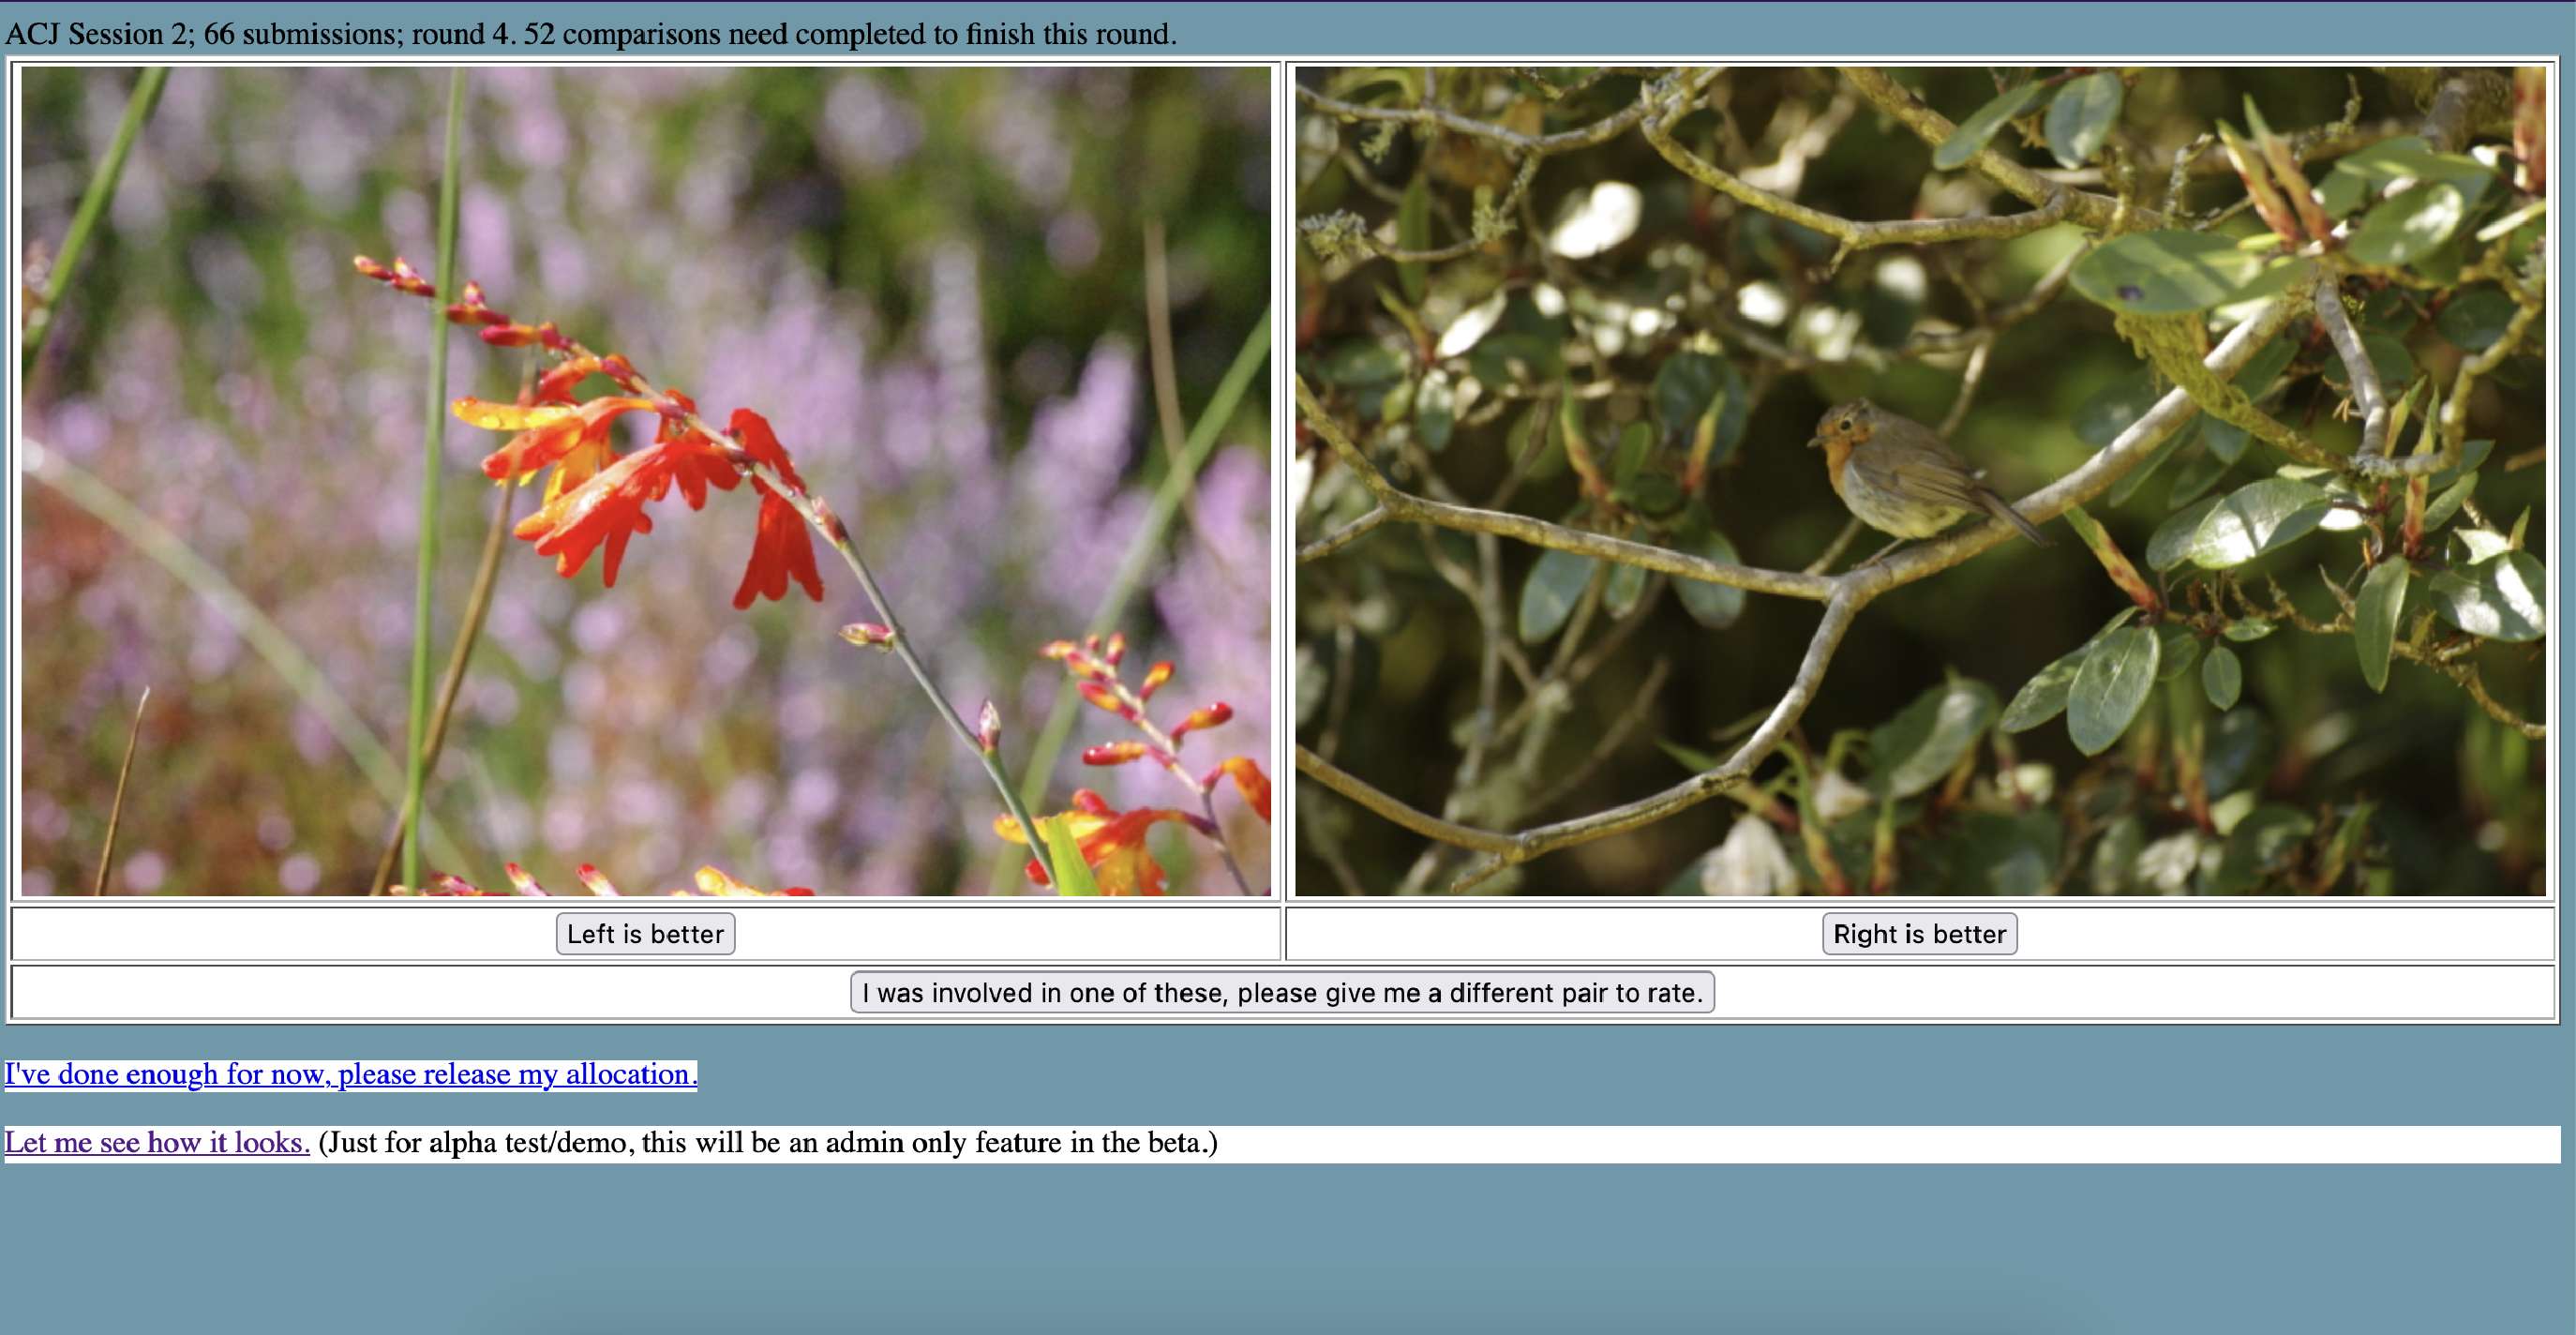
\includegraphics[width=0.95\linewidth]{images/acj-image.pdf}    

    \caption{ Implementation of ACJ \citep{nbarr}. The user is given two different images and is required to decide which one is ``better``.
    }
    \label{fig:acj-image} 
\end{figure}

\section{Aims}
This project aims to develop a JavaScript web application which facilitates the marking of coursework using the method of ACJ. Students should be able to submit their coursework and receive feedback. Evaluators should be allocated pairs of coursework to judge. The judgements should then be used to generate a ranking of the coursework items. Teachers should be able to create new coursework activities for which students submit work.


%==================================================================================================================================
\chapter{Background}

\section{Comparative Judgement}
The method of ACJ is based on the \emph{law of comparative judgement}, a psychophysical law proposed by \citet{thurstone1927law}. This law was intended as a way of measuring the perceived quality of objects such as the excellence of an academic work or the quality of a handwriting specimen. Thurstone posited that when we examine something for comparison we ascribe a value to it denoting its quality. Therefore when we compare two objects we compare these psychological values in order to determine which is “better”. Thurstone derived his own mathematical model for creating a scale of these psychological values based on data derived from many pairwise judgements.

\citet{andrich1978relationships} wrote a Rasch logistic model that was equivalent to Thurstone’s model. This is the model that is more commonly used.

\[log\: odds(A\: beats\: B|v_a,v_b) = v_a - v_b\]

The probability form of the model: 

\[prob(A\: beats\: B|v_a,v_b) = \frac{exp(v_a - v_b)}{1 + exp(v_a - v_b)}\]

Thurstone's method of comparative judgement (CJ) involved comparing every possible pair of scripts and then using the above mathematical model to generate a ranking of the scripts by quality. CJ was first used in an educational setting in a study investigating the assessment of spoken language proficiency \citep{pollitt1996raters} . In this study, five students participated in a video interview to assess their proficiency in speaking English. The video interviews were then shortened into 2-3 minute long segments. Then every possible pairing of video segments was judged by 6 judges. The results showed that CJ could be a reliable way of ranking students’ work by proficiency.

However, using CJ for hundreds or thousands of scripts would be infeasible due to the large of comparisons required. Using CJ for \(n\) number of scripts would require \(\frac{n(n-1)}{2}\) number of comparisons. For example, 500 scripts would require 124750 comparisons. Although CJ could be a reliable method of evaluating student performance, it would impractical to implement.

\section{Introduction of Adaptivity}
This prompted \citet{pollitt2012comparative} to build on the method of CJ by introducing adaptivity. Pollitt realised that more information is gained by comparing scripts that are similar in quality than by comparing scripts that vary greatly in quality. So by only judging the pairings that give the most information, the number of comparisons needed decreases considerably.

The information derived from the result of a single comparison is defined by 
\[I = p(1-p)\]  

The information is the product of the probability of one script winning and the probability of the other script winning. The amount of information gained is maximised when p = 0.5. Pairing scripts so that the probability of one of them winning is between 0.3 and 0.7 will therefore make the judging process more efficient.

\begin{figure}[h]
\begin{center}
    \includegraphics[width=0.65\linewidth]{images/info-pollitt.png}    
    \caption{Information as a function of probability \citep{pollitt2012comparative}}
\end{center}
\end{figure}

\section{Benefits of ACJ}
A study was conducted that investigated the use of ACJ in evaluating writing samples from children aged 9-11 \citep{pollitt2012method}. 1000 writing samples were examined by 54 judges. Due to the inclusion of adaptivity, only 8161 comparisons were made which is a dramatic reduction from the 499500 comparisons needed for CJ. Despite the low number of comparisons, the ACJ study reported a reliability figure of 0.96. This shows that by including adaptivity, the benefits of comparative judgement can still be yielded with a much lower cost. This suggests that ACJ could be a practical alternative to traditional methods of marking.


\section{Application of ACJ in education}
In a study conducted by \citet{bartholomew2019using}, ACJ was used to assess design projects carried out by middle school students. 130 students were instructed to design a travel brochure.
The students’ work was assessed using ACJ and also given a score using a traditional rubric-based approach. The researchers found a significant correlation between the ACJ rank of a project and its rubric-based score. This suggests the validity of ACJ as a method of assessment.

This study also investigated the use of ACJ in formative assessment. The students were split into two groups of 65 and each took part in a peer assessment and feedback session at the midpoint of the design challenge. One group used ACJ for peer assessment and feedback. The other group participated in an informal peer feedback session. The study showed that students who used ACJ at the midpoint of the project performed better than students who did not. This shows that ACJ could potentially be an effective tool for learning as well as assessment.

\section{Pre-existing ACJ Tools}

RM Compare is an online tool, provided by the educational technology company RM, which allows clients to use ACJ for assessment and learning. 

\begin{figure}[h]
\begin{center}
    \includegraphics[width=0.65\linewidth]{images/judging-rm-compare.png}    
    \caption{Judging page in RM Compare's ACJ tool \citep{rmcompare}}
\end{center}
\end{figure}

%==================================================================================================================================
\chapter{Analysis/Requirements}
The main aim of this project was to create a web application that allows markers to assess work from university students using ACJ. The majority of the requirements were gathered in the early stages of the project. They were later refined through weekly meetings with Jeremy Singer, a senior lecturer at the University of Glasgow who proposed this project, and consultation with Niall Barr, a senior learning technology developer at the University of Glasgow who authored the previously mentioned PHP implementation of ACJ. The requirements of this project were explored by writing user stories. Two types of users were decided upon, students and markers. The marker role was used to represent any university staff member. The user stories are listed below.

Each of the requirements were given a priority rating using the MoSCoW method \citep{moscow}. The requirements below have a label 'M', 'S', 'C', or 'W' meaning 'Must have', 'Should have', 'Could have', and 'Would have' respectively.


\section{User Stories}
\textbf{Generic User:}
\begin{itemize}
    \item
        [1] - \textbf{[M]}  As a user, I want to be able to log in using my university email account.
\end{itemize}

\textbf{Student:}
\begin{itemize}
    \item
        [2] - \textbf{[M]} As a student, I want to upload my work, so that it can be graded.
    \item
        [3] - \textbf{[C]} As a student, I want to see a preview of the file that I have uploaded so that I can check that I submitted the correct file.
    \item
        [4] - \textbf{[M]} As a student, I want to be able to remove a file I have submitted in case I have submitted the wrong file.
    \item
        [5] - \textbf{[M]} As a student, I want to see my grade and feedback on my work, so that I can know what I need to improve on.
    \item
        [6] - \textbf{[M]} As a student, I want to see the submission status of all of my assignments so that I know which assignments I still need to submit work for.
    \item
        [7] - \textbf{[M]} As a student, I want to see submission details (deadline, file type, submission instructions) for an assignment so that I know how and when I should submit my work.
    
\end{itemize}
\textbf{Marker:}
\begin{itemize}
    \item
        [8] - \textbf{[M]} As a marker, I want to be able to perform a pairwise comparison of submissions, so that I can rank the submissions in order of quality.
    \item
        [9] - \textbf{[M]} As a marker, I want to have two submissions displayed side-by-side on the screen, so I can easily compare the two.
    \item
        [10] - \textbf{[S]} As a marker, I want to be able to give comments on each submission, so that the student can receive feedback on their work.
    \item
        [11] - \textbf{[M]} As a marker, I want to see a ranking table of all of the submissions, so that I can know how well each student performed.
    \item
        [12] - \textbf{[C]} As a marker, I want to see the submission associated with each entry in the ranking table.
    \item
        [13] - \textbf{[M]} As a marker, I want to create a new assignment, so that my students can submit their work and have it graded using ACJ.
    \item
        [14] - \textbf{[M]} As a marker, I want to set a deadline for an assignment, so that the students can know when their work is due.
    \item
        [15] - \textbf{[M]} As a marker, I want to specify the types of files that can be submitted for an assignment.
    \item
        [16] - \textbf{[M]} As a marker, I want to specify submission instructions so that students know what type of work should be submitted.
    \item
        [17] - \textbf{[M]} As a marker, I want to specify grading instructions so that I can give other markers guidance on how to rank the submissions.
    \item
        [18] - \textbf{[M]} As a marker, I want to add multiple markers to a particular assignment, so that the submissions can be ranked by many people.
    \item
        [19] - \textbf{[S]} As a marker, I want to include students as markers for a particular assignment, so that students can review their peers' work.
    \item
        [20] - \textbf{[M]} As a marker, I want to add multiple students to a particular assignment, so that only my students can submit work.
    
\end{itemize}

\section{Non-Functional Requirements}
\begin{itemize}
    \item
        [21] - \textbf{[M]} The web application has a web-based front-end which the user can interact with using a standard web browser.
    \item
        [22] - \textbf{[W]} The visual layout of the web pages is able to adapt to smaller screens.
\end{itemize}
%==================================================================================================================================
\chapter{Design}
The web application is structured in a 3 tier architecture. It consists of a user interface, ACJ engine and database. The user interacts with the application through their web browser. The ACJ engine sends data to the user’s browser, manages the process of ACJ, and stores or modifies data in the database.

\section{User Interface}

\subsection{Home page}
The user begins at the home page and is asked to sign in. Once signed in, the user is able to navigate to the status page. If the user is a teacher they are also able to access the activity creation page.

\begin{figure}[h]
\begin{center}
    \includegraphics[width=0.65\linewidth]{images/w-home.png}    
    \caption{Wireframe for home page}
\end{center}
\end{figure}

\subsection{Activity creation page}
On the activity creation page a teacher must complete a simple form in order to create a new activity. An activity is an assignment for which students submit work and markers are assigned to judge for. A teacher needs to specify details including submission deadline, students and markers participating, and the number of rounds of ACJ to perform, in order to successfully create a new activity.

\begin{figure}[h]
\begin{center}
    \includegraphics[width=0.45\linewidth]{images/w-create-assignment.png}    
    \caption{Wireframe for activity creation page}
\end{center}
\end{figure}

\subsection{Status page}
The status page displays information about the activities the user is assigned to. The user is shown different information depending on whether they are assigned to submit or judge for a given activity. Users are able to both submit and judge for the same activity. This is to give teachers the option of conducting peer-assessment using ACJ.

The information displayed on the status page also differs depending on what phase an activity is in.

An activity is in the submission phase if its submission deadline has not yet passed. During this time students are shown a link to the submission page so they can upload their work. As judging has not begun, little information is shown to the markers.

Once the submission deadline has passed, the activity enters the judging phase. Students can no longer submit work and markers are given a link to the judging page so they can begin comparing scripts.

After all of the rounds of ACJ have been completed, the activity finally enters the results phase. Students are shown their final rank and comments from markers. Markers are able to view a ranking table of all of the students’ submissions.

\begin{figure}[h]
    \centering
    \begin{subfigure}[b]{0.45\textwidth}
        \includegraphics[width=\textwidth]{images/w-status-student.png}
        \caption{Wireframe of status page for a student}
        \label{fig:syn1}
    \end{subfigure}
    ~ %add desired spacing between images, e. g. ~, \quad, \qquad, \hfill etc. 
      %(or a blank line to force the subfigure onto a new line)
    \begin{subfigure}[b]{0.45\textwidth}
        \includegraphics[width=\textwidth]{images/w-status-marker.png}
        \caption{Wireframe of status page for a marker}
        \label{fig:syn2}
    \end{subfigure}
    ~ %add desired spacing between images, e. g. ~, \quad, \qquad, \hfill etc. 
    %(or a blank line to force the subfigure onto a new line)
    \caption{Wireframes for status page}
\end{figure}

\subsection{Submission page}
The submission page allows students to upload a file containing their work and see a preview of their submitted file. The page also displays some guidance on what kind of work and type of file to submit. This information is defined by the activity creator.

\begin{figure}[h]
\begin{center}
    \includegraphics[width=0.55\linewidth]{images/w-submission.png}    
    \caption{Wireframe for submission page}
\end{center}
\end{figure}

\subsection{Judging page}
The judging page displays two submissions side by side to allow the marker to easily compare the two. Beneath each submission is a text box to enter feedback for the student and a button to allow the judge to select one submission as the winner. Judging instructions from the creator of the activity are also displayed to guide the judge in their decision and remind them of the key criteria being evaluated. After all of the rounds of ACJ have been completed, a ranking table of the submissions is displayed.


\begin{figure}[h]
    \centering
    \begin{subfigure}[b]{0.45\textwidth}
        \includegraphics[width=\textwidth]{images/w-judging.png}
        \caption{Wireframe of judging page}
        \label{fig:syn1}
    \end{subfigure}
    ~ %add desired spacing between images, e. g. ~, \quad, \qquad, \hfill etc. 
      %(or a blank line to force the subfigure onto a new line)
    \begin{subfigure}[b]{0.45\textwidth}
        \includegraphics[width=\textwidth]{images/w-results.png}
        \caption{Wireframe of results page}
        \label{fig:syn2}
    \end{subfigure}
    ~ %add desired spacing between images, e. g. ~, \quad, \qquad, \hfill etc. 
    %(or a blank line to force the subfigure onto a new line)    
\end{figure}

\section{ACJ Engine}

ACJ is conducted in rounds. In each round, the submissions' latest scores and ranks are calculated and pairings are made and shown to judges. Once all of the pairs have been evaluated, the round ends. This process is repeated until the (user-defined) maximum number of rounds has been reached. The algorithm used in this project to optimally pair submissions was originally written by \citet{nbarr:pseudocode} .

At the beginning of the first round, each submission's \lstinline{_latestScore} and \lstinline{rank} are initialised to 0. At the start of every subsequent round, the \lstinline{_latestScore} and \lstinline{rank} for each submission are updated based on the results from the previous round. 

After the latest scores are calculated, the submissions are paired together for comparison. The pairing process starts by creating \lstinline{pairingInfo} objects for each submission. These objects store temporary data which is used to find the most appropriate pair for a given submission.

\begin{figure}[h]
\begin{center}
\includegraphics{images/acj1.class.png}
\caption{Class diagram of implementation by \cite{nbarr:pseudocode}}
\end{center}
\end{figure}


\begin{lstlisting}[language=C, caption={Pseudocode for creating the pairing information by \cite{nbarr:pseudocode}}, captionpos=b]
UpdateRanks(); // make sure submission ranks reflect latest score
targetsList = new array of pairingInfo;
toPairList = new array of pairingInfo;
pairedList = new array of boolean;

foreach(submission)
{
    if(submission has comparisons)
    {
        rank = submission.rank 
        scci = 0 // I can't remember what scci stands for :-(, however this
                 // value is used to bias the choice of next comparison in 
                 // the direction to give balance.
        foreach(submission.comparison)
        {
            compRank = Latest rank of submission with which comparison was done.
            scci += (rank - compRank) / ( 1 + modulus(rank - compRank))
            // this gives similar impact to ranking well above or well 
            // below, but less impact to close rankings.
        }
        cws = rank + scci
    }
    else
    {
       cws = 0; // 'current weighted score' is 0 if no comparisons
    }
    targetRank = cws rounded to nearest integer.
    // TargetList and toPairList differ only in the value of 'score'. 
    targetList.Add(id=submission.id, score=cws, rank=submission.rank, targetRank=targetRank, paired=false);
    toPairList.Add(id=submission.id, score=submission.rank, rank=submission.rank, targetRank=targetRank, paired=false);
    pairedList[submission.id] = false;
}
\end{lstlisting}

After the \lstinline{pairingInfo} objects are generated and stored in \lstinline{toPairList} and \lstinline{targetList}, the lists are sorted by their \lstinline{score} value. Hence, \lstinline{toPairList} is in order of current rank and \lstinline{targetList} is ordered by current weighted score (the ideal current rank of the next comparison). Submissions are then paired up beginning with the \lstinline{pairingInfo} object in the middle of \lstinline{toPairList} and moving outward whilst alternating directions.

\begin{lstlisting}[language=C, caption={Pseudocode for pairing a submission by \cite{nbarr:pseudocode}}, captionpos=b]
pairingInfo = toPairList[nextID]
if(pairedList[pairingInfo.id] == false) // skip if it's already paired
{
    // indicate it is paired, a simple way of avoiding pairing with itself.
    pairedList[pairingInfo.id] = true
    // start search for pairing at targetRank
    suggestID = pairingInfo.targetRank;
    while(suggestID is valid and one or more of:
          targetsList[suggestID] has been paired
          or targetsList[suggestID] is this submission
          or targetsList[suggestID] has already been compaired with this submission)
    {
         suggestID is next choice, starting from original target and working outwards.
    }
    if(suggestID == false)
    {
        Do the same as above again, but allowing duplicate comparisons.
    }
    if(suggestID is valid) // it always is
    {
        Add the pairing to the pairings array, and mark the target as paired in pairedList
    }
}
\end{lstlisting}

After all of the submissions are paired together, the pairings are assessed by the judges. The \lstinline{_latestScore} and \lstinline{rank} for each submission are recalculated based on the results from all previous comparisons. The algorithm for calculating the score for a particular comparison differs depending on the round number. The submission's \lstinline{_latestScore} is set to the sum of the scores of all its past comparisons divided by the total number of comparisons it has had.

\begin{lstlisting}[language=C, caption=Calculating the score for a submission for a particular round, captionpos=b]
if(round <= 4){
    if(won comparison){
        score = 1;
    }
    else{
        score = -1;
    }
}
else if(round <= 8){
    if(won comparison){
        score = pairRank;
    }
    else{
        score = -1 * (number of submissions - pairRank);
    }
}
else{
    rmsRankDiff = sqrt((pairRank-thisRank)*(pairRank-thisRank));
    if(won comparison){
        score = thisRank + thisRank/rmsRankDiff;
    }
    else{
        score = thisRank - thisRank/rmsRankDiff;
    }
}
\end{lstlisting}

\section{Database}
In order for ACJ to work correctly, data about users, submissions, and comparisons must be securely stored. A relational database was chosen instead of a NoSQL database as the type of data needed to be stored could be easily structured. The structure of the tables can be seen in figure \ref{fig:er}.

The acjComparison table stores details about pairs of submissions. The acjResource table stores data about activities. "Resource" and "activity" are used interchangeably in this project.


\begin{figure}[h]
\begin{center}
    \includegraphics[width=0.95\linewidth]{images/ER-diagram.png}    
    \caption{ER diagram}
    \label{fig:er}
\end{center}
\end{figure}

%==================================================================================================================================
\chapter{Implementation}

\section{Overview}

Node.js and the Express.js framework were used to build the fundamental features of the web application. An SQLite database was used in this project. However, due to its limitations in terms of database size and capacity for concurrent users, it unsuitable for use in production\citep{sqlite}. Other database systems should be used instead such as PostgreSQL or MySQL.

\section{Front-end}
The front-end was initially developed using the JavaScript React library. Originally, the project consisted of two apps (React front-end and Express back-end) running simultaneously. But this caused complications when configuring the log in system to use OpenID Connect. To resolve this, the React application was removed and the front-end was designed using Handlebars.js, a simple templating language.

The Bootstrap CSS framework was used to provide simple styling to the web pages and structure important pages, such as the judging page, appropriately. To help markers examine submissions of source code, the highlight.js library was used to highlight code. This library automatically detects the programming language being used and highlights the appropriate text.

\begin{figure}[h]
\begin{center}
    \includegraphics[width=0.80\linewidth]{images/judging.png}    
    \caption{Judging page. Built using Bootstrap, highlight.js, and Handlebars.js}
\end{center}
\end{figure}


\section{OpenID Connect with Microsoft}

The sign in system was built to use the OpenID Connect authentication protocol with the Microsoft identity platform. This allows users to log in using their university email credentials provided that their university has a Microsoft 365 subscription. Consequently, new users do not need to go through the process of creating a new account. This simplifies the log in process and makes the web application more easily accessible for university staff and students.

To use OpenID Connect with Microsoft, the web application needed to be registered in the Microsoft Azure portal \citep{openid:node}. The application's registration details and the @azure/msal-node JavaScript library were used together to make the appropriate requests to the Microsoft authorisation server.

\subsection{Sign In Flow}

User clicks 'sign in with your university email'.

\begin{figure}[h]
\begin{center}
    \includegraphics[width=0.75\linewidth]{images/home-before.png} 
    \caption{Home page when user is not signed in.}
\end{center}
\end{figure}

The ACJ web application redirects the user to the Microsoft Log in page.

Once the user enters their email credentials, the Microsoft authorisation server redirects the user back to the ACJ web application and sends back an authorisation code.

The ACJ web application sends the authorisation code, client ID, and client secret to the authorization server

The authorisation server verifies the data and sends back an access token, ID token, and account information. The account information contains the user’s email address which is used why the ACJ application to determine if the user is a student or marker.
	
The user is now signed in.
	

\begin{figure}[h]
\begin{center}
    \includegraphics[width=0.85\linewidth]{images/convergence-scenarios-webapp.pdf}  
    \caption{OpenID Connect sign-in flow \citep{openid}}
\end{center}
\end{figure}



\section{ACJ}

ACJ is performed in rounds. In each round, all of the submissions are paired together and then pairings are made available to the markers for judgement.

The process of pairing involves: 
\begin{itemize}
  \item calculating the latest score and rank for each submission
  \item generating temporary pairing information for each submission
  \item pairing submissions using temporary pairing information
  \item store the pairings in the database
\end{itemize}
    



\begin{lstlisting}[language=C, caption=JavaScript code for calculating the scores for each submission, captionpos=b]
this.updateRanks();
for(let pID in this.papers){
    let sc = 0;
    let cmprank;
    if(this.papers[pID].comparisons.length){
        for(let cmp of this.papers[pID].comparisons){
            if(round <= 4){
                cmprank = this.papers[cmp.withID].rank;
                if(cmp.won){
                    sc += 1;
                }
                else{
                    sc -= 1;
                }
            }
            else if(round <= 8){
                cmprank = this.papers[cmp.withID].rank;
                if(cmp.won){
                    sc += cmprank;
                }
                else{
                    sc -= (Object.keys(this.papers).length - cmprank);
                }
            }
            else{
                cmprank = this.papers[cmp.withID].rank;
                let thisrank = this.papers[pID].rank;
                let rmsRankDiff = Math.sqrt((cmprank-thisrank)*(cmprank-thisrank));
                if(cmp.won){
                    sc += thisrank + thisrank/rmsRankDiff;
                }
                else{
                    sc += thisrank - thisrank/rmsRankDiff;
                }
            }
        }
        sc = sc / this.papers[pID].comparisons.length;
    }
    this.papers[pID].addScore(round, sc);
}
\end{lstlisting}

\begin{lstlisting}[language=C, caption=JavaScript code for generating the temporary pairing info for submissions, captionpos=b]
this.updateRanks();
let targetsList = [];
let toPairList = [];
let pairedList = {};

for(let pID in this.papers){
    //Calculate a score for each paper based on its past comparisons
    let cws = 0;
    if(this.papers[pID].comparisons.length > 0){
        let n = 0;
        let rank = this.papers[pID].rank;
        let scci = 0;
        for(let c of this.papers[pID].comparisons){
            n++;
            let compRank = this.papers[c.withID].rank;
            scci += ((rank - compRank) / (1 + Math.sqrt((rank-compRank)*(rank-compRank))));
        }
        cws = rank + scci;
    }

    targetsList.push({
        id: pID,
        score: cws,
        rank: this.papers[pID].rank,
        targetRank: parseInt(Math.floor(cws+0.5)),
        paired: false
    });
    toPairList.push({
        id: pID,
        score: this.papers[pID].rank,
        targetRank: parseInt(Math.floor(cws+0.5)),
        paired: false
    });
    pairedList[pID] = false;
}
targetsList.sort(cmp2);//sorting by score
toPairList.sort(cmp2);//sorting by score
\end{lstlisting}


\begin{lstlisting}[language=C, caption=JavaScript code for pairing up submissions using pairing info, captionpos=b]
 const s = toPairList.length;
let pairings = [];
let nextID = nextAlternating(false, s);
while(nextID !== false){
    let pl = toPairList[nextID];
    //pair the paper if it is unpaired
    if(pairedList[pl.id] === false){
        pairedList[pl.id] = true;
        let suggestID = nextOffsetAlternating(false, pl.targetRank, s);
        while((suggestID !== false) && ((pairedList[targetsList[suggestID].id]) || (targetsList[suggestID].id==pl.id) || (this.papers[pl.id].countComparisons(targetsList[suggestID].id)))){
            suggestID = nextOffsetAlternating(suggestID, pl.targetRank, s);
        }
        if(suggestID === false){
            suggestID = nextOffsetAlternating(false, pl.targetRank, s);
            while((suggestID !== false) && (targetsList[suggestID].id==pl.id)){
                suggestID = nextOffsetAlternating(suggestID, pl.targetRank, s);
            }
        }
        if(suggestID !== false){
            pairedList[targetsList[suggestID].id] = true;
            pairings.push([pl.id, targetsList[suggestID].id]);
        }
    }
    nextID = nextAlternating(nextID, s);
}
return pairings;
\end{lstlisting}

The judging process involves:
\begin{itemize}
  \item Searching the database for a pair that has not been evaluated.
  \item If a pair is found then it is shown to the marker.
  \item When a decision is made it is recorded in the database and a new pair (if available) is shown to the marker.
  \item This cycle continues until all pairings have been judged.
  \item If the maximum number of rounds has not been reached then the pairing process for the next round begins.
  \item If the maximum number of rounds has been reached, then the table of rankings is displayed.
\end{itemize}

\begin{figure}[h]
\begin{center}
    \includegraphics[width=0.85\linewidth]{images/results.png}  
    \caption{Table ranking page after all rounds of ACJ have been completed}
\end{center}
\end{figure}

%==================================================================================================================================
\chapter{Evaluation} 

\section{Think Aloud Study}

A think aloud study was conducted with Niall Barr (the developer of the PHP implementation of ACJ). He was instructed to explore the web application on his own and voice his thought process throughout. Barr was asked to participate in this study because his knowledge of ACJ and experience of writing ACJ software would likely provide a deeper insight into the quality of the project.

\subsection{Tasks and Comments}

The web application was run on a laptop using macOS. The web application was accessed using the Firefox web browser. This fulfills requirement 21.

Barr began on the home page which only shows a "sign in" link. He commented that the page should let the user know that their university email will be used to log in and suggested changing the page to say "Log in with your university ID".

Barr clicked on "sign in" and was redirected to the Microsoft log in page. After entering his credentials he was redirected back to the ACJ web application. This shows the fulfillment of requirement 1.

Now logged in, he navigated to the "create activity" page and began filling out the activity form. When he reached the "submission type" field, he was not sure what type of information to enter and asked if their are specific limitations or if it is just guidance for students.

For the "List of Students (CSV)" and "List of Markers (CSV)" fields he uploaded CSV files with fake data that were created beforehand.

He commented that in his ACJ system the teacher can stop the judging at any point whereas with my system the number of rounds of ACJ is defined by the user when an activity is created.

He submitted the activity creation form and then navigated to the status page. He expected to see the activity he had just created but instead was shown a blank status page. This was because his email address was not included in the student or marker CSV files uploaded on the activity creation page.


As my email was included in the student and marker CSV files, I suggested that Barr sign out and sign in with my account.

After signing out and signing in with my account, he went to the status page and was able to see the activity he created earlier. The successful creation of the activity shows that requirement 13, 14, 15, 16, 17, 18, 19, and 20. As my email was included in the student and marker CSV files, both the marking and submission information which fulfils requirement 6.

Barr navigated to the submission page for the activity he created. The page displayed submission details and a box for uploading a file. He successfully uploaded a file and was redirected back to the status page. This shows that requirement 2 and 7 are fulfilled.

Barr asked if there activity deadlines could be changed. I replied that they can't be.

Barr then started judging for an activity that was created and populated with submissions before the study. After he made his first judgement an error occurred in the system and I began debugging the system.

Barr commented that the system so far looked nice. He asked if the comments box on the judging page was for the marker for when they see the same submission again or for the student. I replied that the comments go to the student.

Once the bug was fixed, Barr began judging again thus fulfilling requirement 8. Some submissions contained a lot of text which did not fit completely in the frame on the judging page. Barr used the scroll bar to see the rest of the submission. He then commented that he uses a JavaScript library which allows the user to resize frames.

Barr commented that the judgement page in particular is nice and clear.

He then suggested that users who create activities should be included in the markers and/or students list by default. This is because administrators would be the people who create activities and although they would not be involved in the marking, they still need to view details about the activity. A third role of "creator" or "admin" could be added.

Barr then asked to view the results page that appear after all of the ACJ rounds are completed. After quickly finishing the judging for an activity, the results page appeared displaying a table of the user IDs in rank order. This fulfils requirement 11. He mentioned that if the project were to be used in production, there would need to be a feature for the administrators to easily take in the data from the results of an activity. One possible method would be allowing the results to be exported as a Microsoft Excel spreadsheet.

Barr's final comment was that the system looked good overall.


\section{Comparison with Pre-existing Projects}

Niall Barr's vs mine

- comparing images vs source code files

- no comments vs comments

- can view ranking whenever vs only view ranking after pre-defined number of rounds completed

% - no log in vs log in

% - no activity creation or work submission vs activity creation and work submission




%==================================================================================================================================
\chapter{Conclusion}    

\section{Summary}
This project aimed to build a JavaScript web application that allows users to assess student work using the method of ACJ.


\section{future work}
-Introduce an admin role

-Add more supported file formats

-Make web pages adapt to smaller screens

%==================================================================================================================================
%
% 
%==================================================================================================================================
%  APPENDICES  

\begin{appendices}

\chapter{Appendices}



\end{appendices}

%==================================================================================================================================
%   BIBLIOGRAPHY   

% The bibliography style is abbrvnat
% The bibliography always appears last, after the appendices.

\bibliographystyle{abbrvnat}

\bibliography{l4proj}

\end{document}
